\chapter{柯西积分公式及应用}

\section{全纯函数的积分表示}
可求长曲线. 对$[a,b]$ 做分割$\lambda : a = t_0 < t_1 < ... < t_n = b$, 取$\xi_i \in [t_{i-1}, t_i], i=1,...,n$.
做Riemann和:$\sum_{k=1} ^{n} f(\xi_k) (z_k - z_{k-1})$. 设$d=\Vert  \lambda \Vert$. $d \rightarrow 0$时,Riemann和有极限(略去). 记$\Delta z_k = z_k - z_{k-1}$. 故
\begin{align*}
R(f) &= \sum_{k=1}^{n}f(\xi_k) - \Delta z_k \\
&= \sum_{k=1}^{n} (u(\xi_k) + i v(\xi_k))(\Delta x_k + i \Delta y_k) \\
&= \sum_{k=1} ^{n} u(\xi_k) \Delta x_k - \sum_{k=1}^{n} v(\xi_k) \Delta y_k + i [(\sum_{k=1}^{n} u(\xi_k) \Delta y_k + \sum_{k=1}^n v(\xi_k) \Delta x_k]
\end{align*}
故当u于v在$\gamma$上连续时,令$d \rightarrow 0$,则f的Riemann和趋于曲线积分:$\int_{\gamma} (udx - vdy) + i \int_{\gamma}vdx-udy$, 即: 
\begin{mypro}
	$f = u+iv$在可求长曲线$\gamma$上连续,则有:
	$$\int_\gamma f(z) dz = \int_\gamma (udx-vdy) + i\int_\gamma (vdx+udy).$$
\end{mypro}
\begin{mypro}
	若$z=\gamma(t)$为光滑的曲线,$f$在$\gamma$上连续,则:$\int_\gamma f(z)dz = \int_a^b f(\gamma(t))\gamma'(t) dt$
\end{mypro}
\begin{proof}
	由于$z=\gamma(t)$ 故$\gamma'(t)=x'(t) + i y'(t)$.
	
	而$dx=x'(t)dt, dy = y'(t)dt$,代入3.1.1即可得证.
\end{proof}

\begin{mypro}
	若$f, g$在可求长曲线$\gamma$上连续,则:
	\begin{enumerate}[i)]
		\item $\int_\gamma f(z)dz = -\int_\gamma f(z)dz$
		\item $\int_\gamma (\alpha f(z) + \beta g(z)) dz = \alpha \int_\gamma f(z) dz + \beta \int_\gamma g(z) dz$, \quad $\alpha, \beta \in \mathbb{C}$
		\item $\int_\gamma f(z) dz = \int_{\gamma_1} f(z) dz + \int_{\gamma_2} f(z) dz$. 其中$\gamma_1 \cup \gamma_2 = \gamma$, $\gamma_1 \cap \gamma_2 = \emptyset $
	\end{enumerate}
\end{mypro}

\begin{mypro}[长大不等式]
	
	若曲线$\gamma$的长度为$L$, $M = \max_{z \in \gamma} \vert f(x) \vert$,
	则$ \vert \int_\gamma  f(z) dz \vert \leq ML$
\end{mypro}
\begin{proof}
	直接利用Riemann和验证即可.
\end{proof}

\section{\emph{Caucy}积分定理}
\begin{mypro}[\emph{Caucy}]
	设$D$为$\mathbb{C}$中的单连通域,$f \in H(D)$,且$f' \in C(D)$, 则对$D$中的任意可求长闭曲线$\gamma$,均有$\int_\gamma f(z) dz = 0$.
\end{mypro}
\begin{proof}
	由Green公式以及C-R方程直接得到.
\end{proof}

\begin{mypro}
	设$f$是域$D$中的连续函数,$\gamma$是$D$内可求长曲线,则$\forall \varepsilon > 0$, 存在一条$D$上的折线$P$使得:
	\begin{enumerate}[(i)]
		\item $P$和$\gamma$有相同的起点和终点,$P$的其他顶点在$\gamma$上.
		\item $\vert \int_\gamma f(z) dz - \int_Pf(z) dz \vert < \varepsilon $.
	\end{enumerate}
\end{mypro}
\begin{proof}
	见chb笔记.
\end{proof}

\begin{mypro}[\emph{Cauchy-Goursat}]
	设$D$为$\mathbb C$中的单连通域,若$f \in H(D)$, 则对于$D$中的任意可求长闭曲线$\gamma$,均有$\int_\gamma f(z) dz = 0$.
\end{mypro}
\begin{proof}
	利用上一定理3.2.2,见chb笔记.
\end{proof}

但定理3.2.3的条件仍可以再做减弱:
\begin{mypro}
	设$D$是简单可求长闭曲线$\gamma$的内部,若$f \in H(D) \cap C(\bar{D})$,则$\int_\gamma f(z) dz = 0$.
\end{mypro}
这一定理的证明现在无法进行,我们对其弱化进行证明:

\addtocounter{mypro}{-1}
\begin{mypro}[*]
	设$\gamma$为$\mathbb{C}$上分段光滑的可求长闭曲线,记$D$为$\gamma$围成的区域内部,且存在$D$中的点$z_0$,使得任意一条从$z_0$发出的射线与$\gamma$有且只有唯一交点,若$f \in H(D) \cap C(\bar{D})$,则$\int_\gamma f(z) dz = 0$.
\end{mypro}

\begin{figure}[h]
	\centering
	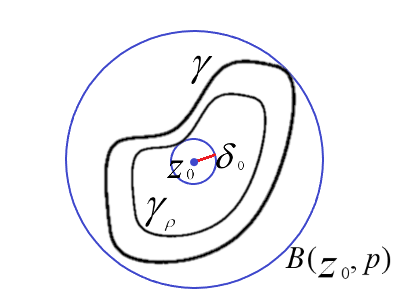
\includegraphics[scale=0.4]{chp3_p2}
\end{figure}

\begin{proof}
	由于我们增加的条件,故$\gamma$可写为$z = z_0 + \gamma(t)$, $a \leq t \leq b$.
	记$p = \max_{a \leq t \leq b} \vert \lambda (t) \vert, q = \max_{a \leq t \leq b} \vert \lambda'(t) \vert$. 闭区间分段连续保证有最值(光滑保证)
	由于$f$在$\bar{D}$上连续,故一致连续,即$\forall \varepsilon > 0$, 存在$\delta > 0$ $s.t. z_1, z_2 \in \bar{D}, \vert z_1 - z_2 \vert < \delta$ 时,$\vert f(z_1) - f(z_2) \vert < \varepsilon$
	取 $\delta_0 = \min \{ \delta, p \}$, 故$\frac{\delta_0}{p} <1 $, 取 $\rho$ $ s.t. 1 - \frac{\delta_0}{p} < \rho < 1$
	
	记曲线$\gamma_\rho: z = z_0 + \rho \lambda(t), a \leq t \leq b$, 则$\gamma_\rho \subset D$. 由定理3.2.3得 $\int_{\gamma_\rho} f(z)dz = \int_a^b f(z_0 + \rho \lambda(t)) \rho \lambda'(t) dt = 0 \Rightarrow \int_a^b f(z_0 + \rho \lambda(t)) \lambda'(t) dt = 0$.
	由于$\vert (z_0 + \rho \lambda(t)) - (z_0 + \lambda(t)) \vert = (1 - \rho) \vert \lambda(t) \vert \leq (1-\rho) p < \delta_0 < \delta$
	故$\vert f(z_0 + \rho \lambda(t)) - f(z_0 + \lambda(t)) \vert < \varepsilon$.
	故
	\begin{align*}
	\vert \int_\gamma f(z) dz \vert &= \vert \int_a ^b f(z_0 + \lambda(t)) \lambda'(t) dt \vert \\
	&= \vert \int_a^b [f(z_0 + \lambda(t)) - f(z_0 + \rho \lambda(t))] \lambda'(t) dt \vert\\
	&\leq \int_a^b \vert f(z_0 + \rho \lambda(t)) - f(z_0 + \lambda(t)) \vert \vert \lambda'(t) \vert dt\\
	&< \varepsilon q(b-a)
	\end{align*}
	由$\varepsilon$的任意性得$\int_\gamma f(z) dz = 0$.
	
\end{proof}




\begin{mypro}[多连同区域的\emph{Cauchy}积分公式]  略.
\end{mypro}

\begin{figure}[h]
	\centering
	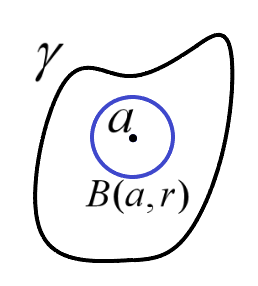
\includegraphics[scale=0.4]{chp3_p3_1.png}
\end{figure}
\begin{eg}
	计算积分$\int_\gamma \frac{dz}{(z - a)^n}, n \in \mathbb{Z}$ , a 在$\gamma$ 围成区域内部.
\end{eg}
\begin{jie}
	
	故$\int_\gamma \frac{dz}{(z-a)^n} = \int_{|z-a| = r} \frac{dz}{(z-a) ^n}  = \int_0 ^ \pi \frac{r e ^{i \theta} i d \theta}{(re^{i \theta})^n} = i r^{1-n} \int_0^{2\pi} (e^{i\theta})^{1-n} d \theta$.
	
	若$n \neq 1$, 则$\int_0 ^{2\pi} (e^{i \theta})^{1-n} d\theta$为复积分,值为0;
	若$n=1$,则$\int_\gamma \frac{dz}{(z - a)^n} = i \int_0 ^{2\pi} 1 d\theta = 2\pi i$.
\end{jie}


\begin{figure}[h]
	\centering
	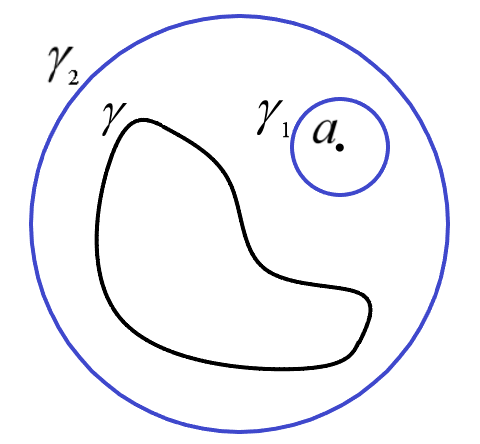
\includegraphics[scale=0.25]{chp3_p3_2.png}
\end{figure}

\begin{eg}
	计算积分$\int_\gamma \frac{dz}{z - a}$.
\end{eg}
\begin{jie}
	\begin{enumerate}[(1)]
		\item a在$\gamma$围成区域内部,结果同上,$\int_\gamma \frac{dz}{z-a} = 2\pi i$.
		\item a在$\gamma$围成区域外部,故$\int_\gamma \frac{dz}{z-a} = \int_{\gamma_2} \frac{dz}{z -a} - \int_{\gamma_1} \frac{dz}{z-a} = 0$.
	\end{enumerate}
\end{jie}


\section{全纯函数的原函数}
\begin{mypro}
	设f在域D中连续,且对于D中任意可求长闭曲线,均有$\int_\gamma f(z) dz = 0$, 那么$F(z) = \int_{z_0}^{z} f(\xi) d\xi$ 是D上的全纯函数且在D中有$F'(z) = f(z)$.
\end{mypro}
\begin{mypro}
	见chb笔记,略.
\end{mypro}

\section{\emph{Cauchy}积分公式的一些重要推论}

\begin{mypro}[Liouville定理]
	有界整函数必为常数
\end{mypro}
\begin{proof}
	设$f$为一有界整函数,其模的上界设为$M$.即$\forall z\in\mathbb{C}$,
	有$|f(z)|\leq M$,任取$a\in\mathbb{C}$,在$\partial$$B(a,R)$上由$Cauchy$不等式得$\displaystyle{|f(a)|\le\frac{M}{R}}$,
	$\forall R>0$.令$R\rightarrow\infty$得$|f'(a)|=0\Rightarrow f'(a)=0\forall a\in\mathbb{C}$故$f$为常数.
\end{proof}

\begin{mypro}[代数基本定理]
	任意复系数多项式$P(z)=a_{0}z^{n}+a_{1}z^{n-1}+\dots+a_{n}$\quad$(a_{0}\neq0)$在$\mathbb{C}$中必有零点
\end{mypro}
\begin{proof}
	略,见$chb.$和史济怀\quad$\displaystyle{(F(x)=\frac{1}{P_{z}})}$
\end{proof}

\begin{mypro}[Morera]
	若$f$是域$\mathbb{D}$上的连续函数,且沿$\mathbb{D}$内任意可求长闭曲线上的积分是0,那么$f$在$\mathbb{D}$上解析
\end{mypro}
\begin{proof}
	见$chb.$笔记
\end{proof}

\subsection*{习题}
\begin{eg}
	{\rm Liouville}定理的另一个证明
\end{eg}
\begin{proof}
	设$f$是有界整函数,$z_{1},z_{2}$是$B(0,r)$中的任意两点,则:
	\begin{align*}
	\int_{|z|=r}\frac{f(z)}{(z-z_1)(z-z_2)}dz
	&=\frac{1}{z_1-z_2}
	\left(\int_{|z|=r}\frac{f(z)}{z-z_1}dz-\int_{|z|=r}\frac{f(z)}{z-z_2}dz\right)\\
	&=\frac{1}{z_2-z_1}\left(f(z_1)-f(z_2)\right)
	\end{align*}
	由于$f$有界.故存在$M>0,s.t\quad|f(z)|\leq M,\forall z\in \mathbb{C}$\\
	故:
	\begin{align*}
	\left|\int_{|z|=r}\frac{f(z)dz}{(z-z_1)(z-z_2)}\right|
	&\leq\int_0^{2\pi}\left|\frac{f(z)\cdot zd\theta}{(z-z_1)(z-z_2)}\right|\\
	&\leq\int_0^{2\pi}\frac{M\cdot r}{|z-z_1|\cdot|z-z_2|}d\theta\\
	&\rightarrow 0\quad(r\rightarrow\infty)
	\end{align*}
	故:$\displaystyle{\int_{|z|=r}\frac{f(z)dz}{(z-z_1)(z-z_2)}=0}$. \quad 故:$\displaystyle{f(z_1)=f(z_2)}$.\\
	由于$r,z_1,z_2$的任意性,故$f(z)$为常值函数.
\end{proof}

\begin{eg}
	设$f$为整函数,若当$z\rightarrow+\infty$时.$f(z)=0(|z|^\alpha)\quad\alpha\geq0$.证明$f$是次数不超过$[\alpha]$的多项式
\end{eg}
\begin{proof}
	记.$k=[\alpha]+1$\\
	$\displaystyle{\Rightarrow\lim\limits_{z\to\infty}\frac{f(z)}{z^k}=0}$.
	由于$\displaystyle{f^{(k)}(z)=\frac{k!}{z\pi i}\int_{|z|=R}\frac{f(\xi)}{(\xi-z)^{k+1}}d\xi}$.
	故$\forall\epsilon>0.\exists R, s.t\quad r>R$有$\displaystyle{\left|\frac{f(z)}{z^k}\right|<\epsilon,z\in B(0,r)}$.(令$r\rightarrow\infty$)\\
	$\displaystyle{\Rightarrow\left|f^{(k)}(z)\right|\leq\frac{1}{2\pi}\int_{|z-\xi|=r}\left|\frac{f(\xi)}{(\xi-z)^{k+1}}\right|d\xi=r\epsilon}$.
	故$f^{(k)}\equiv0$.
\end{proof}

\begin{eg}
	设$f$为整函数,如果$f(\mathbb{C})\subset\{z\in\mathbb{C};I\!m\ z>0\}$,证明$f$为常值函数.
\end{eg}
\begin{proof}
	$\Rightarrow \forall z\in \mathbb{C}, |f(z)+i|\geq 1$ \quad 令$\displaystyle{g(z)=\frac{1}{f(z)+i}}$\\
	故$g(z)\in H(\mathbb{C})$. 并且\quad$|g(z)|\leq1$.故$g$为常值函数,故$f$为常值函数
\end{proof}

\begin{eg}
	设$f$为整函数.如果$f(\mathbb{C})\subset\mathbb{C}\backslash[0,1]$.证明:$f$为常值函数.
\end{eg}
\begin{proof}
	令$\displaystyle{g(z)=\frac{f(z)}{1-f(z)}}$.若$g(z)=r\in\mathbb{R}^+$.则$\displaystyle{f(z)=\frac{r}{r+1}\in[0,1]}$.矛盾\\
	故$g(z)\subset\mathbb{C}\backslash[0,+\infty)$.设$h(z)=\sqrt{g(z)}$.显然$h$也为整函数.\\
	故$h(\mathbb{C})\subset\{z\in\mathbb{C};I\!m\ z>0\}$.故$h$为常值函数.故$f$为常值函数
\end{proof}

\begin{eg}[更强形式的Morera]
	设$f$是域$\mathbb{D}$上的连续函数,若对于任意边界和内部位于$\mathbb{D}$中三角形域$\triangle$,
	总有$\int_{\partial\triangle}f(z)dz=0$.证明$f\in H(\mathbb{D})$.
\end{eg}
\begin{proof}
	思路同\emph{Cauchy-Gousart}.此处省略
\end{proof}

\begin{eg}
	$\displaystyle{\int_{|z|=a}\frac{e^z}{z^2+a^2}.(a\in\mathbb{(R)^+})}$.
\end{eg}
\begin{jie}
	\begin{align*}
	&\int_{|z|=a}\frac{e^z}{z^2+a^2}\\
	=&\int_{|z|=a}\frac{e^z}{(z+ai)(z-ai)}dz=\frac{1}{2ai}\int_{|z|=a}\left(\frac{e^z}{z-ai}-\frac{e^z}{z+ai}\right)dz\\
	=&\frac{2\pi i}{2ai}\left((e^z)|_{z=ai}-(e^z)|_{z=-ai}\right)=\frac{2\pi i}{a}\sin a
	\end{align*}
\end{jie}

\begin{eg}
	设$f\in H(\{z:r<|z|<+\infty\})$.且$\lim\limits_{z\rightarrow\infty}z\cdot f(z)=A$.
	证明:$\displaystyle{\int_{|z|=R}f(z)dz\rightarrow 2\pi iA}$,\\$(R\rightarrow\infty)$.
\end{eg}
\begin{proof}
	由条件得.$\forall\epsilon>0,\exists R_0>r,s.t.|z|\geq R_0$时,有$|zf(z)-A|<\epsilon$.
	故:
	\begin{align*}
	\left|\int_{|z|=R}f(z)dz-2\pi iA\right|
	&=\left|\int_{|z|=R}f(z)dz-\int_{|z|=R}\frac{A}{z}dz\right|\\
	&=\left|\int_{|z|=R}(f(z)-\frac{A}{z})dz\right|\leq\int_{|z|=R}\left|f(z)-\frac{A}{z}\right|dz\\
	&\leq\int_{|z|=R}\frac{\epsilon}{R}dz=2\pi\epsilon
	\end{align*}
\end{proof}
\begin{eg}
	无界区域的\emph{Cauchy}积分公式:\\
	设$\gamma$为$\mathbb{C}$中的有限的可求长闭曲线,设$\gamma$围成的区域为$D$.记$\Omega=\mathbb{C}\backslash(D\cup \gamma)$\\
	设$f\in C(\Omega\cup \gamma)\cap H(\Omega)$,且$\lim\limits_{|z|\rightarrow\infty}f(z)=f(\infty)\in\mathbb{C}$.
	则$\displaystyle{f(z)=f(\infty)-\frac{1}{2\pi i}\int_{\gamma}\frac{f(\xi)}{\xi-z}d\xi}$.
\end{eg}
\begin{proof}
	任取$\displaystyle{z\in\Omega.\exists R>0,s.t.\ \gamma\cup\{z\}\subset B(0,R)}$.\\
	由$\displaystyle{f(z)=\frac{1}{2\pi i}\int_{|z|=R}\frac{f(\xi)}{\xi-z}d\xi-\frac{1}{2\pi i}\int_{\gamma}\frac{f(\xi)}{\xi-z}d\xi}$.\\
	取$\displaystyle{\xi\in\{z:|z|=R\}}$.令$\displaystyle{R\rightarrow+\infty,\ \frac{f(\xi)}{\xi-z}\cdot\xi\ \rightarrow f(\infty)}$\\
	由前例子可得$\displaystyle{\frac{1}{2\pi i}\int_{|z|=R}\frac{f(\xi)}{\xi-z}d\xi\ \rightarrow f(\infty),\ R\rightarrow+\infty}$\\
	故$\displaystyle{f(z)=f(\infty)-\frac{1}{2\pi i}\int_\gamma\frac{f(\xi)}{\xi-z}d\xi}$
\end{proof}

\begin{eg}[Painlev\'e原理]
	设$D$为域,$\gamma_1,\gamma_2\dots \gamma_n$是$D$中的$n$条可求长闭曲线,
	若$\displaystyle{f\in C(D)\cap H(D\backslash \mathop{\bigcup}\limits_{k=1}^{n}\gamma_k)}$则$f\in H(D)$.
\end{eg}
\begin{proof}
	利用定理$3.2.4$及\emph{Morera}定理即可,略
\end{proof}

\section{最大模原理}
\begin{mypro}[平均值定理]
	设$f\in H(B(z_0,r))\cap C(\,\overline{B(z_0,r)}\,)$.则:$\displaystyle{f(z_0)=\frac{1}{2\pi}\int_0^{2\pi}f(z_0+re^{i\theta})d\theta}$.
\end{mypro}
\begin{proof}
	由\emph{Cauchy}积分公式得$\displaystyle{f(z_0)=\frac{1}{2\pi i}\int_{|z-z_0|=r}\frac{f(\xi)}{\xi-z_0}d\xi}$\\
	记$\displaystyle{\xi=z_0+re^{i\theta}\Rightarrow d\xi=ire^{i\theta}d\theta=i(\xi-z_0)d\theta}$\\
	$\displaystyle{\Rightarrow f(z_0)=\frac{1}{2\pi}\int_0^{2\pi}f(z_0+re^{i\theta})d\theta}$
\end{proof}
\begin{mypro}[最大模定理]
	设$\Omega$为区域$f\in H(\Omega)$.则$|f|$在$\Omega$内有最大值当且仅当$f$为常函数
\end{mypro}
\begin{proof}
	此处给出利用区域连通性与平均值原理的证法,见\emph{chb}笔记.略\\
	具体可见方企勤\emph{《复变函数》}
\end{proof}

\begin{mypro}
	设$D\subset\mathbb{C}$为有界域.设$f$为非常值函数.
	$f\in H(D)\cap C(D)$.则$f$的最大模在且只在$\partial D$上取到
\end{mypro}
\begin{proof}
	由定理\emph{3.6.2}可直接得到.略
\end{proof}

\begin{mypro}[Schwarz引理]
	设$f\in H(B(0,1))$,且有$\forall z\in B(0,1),\ |f(z)|\leq1,\ f(0)=0$.
	则$\forall z\in B(0,1)$有$|f(z)|\leq|z|,|f'(0)|\leq1.$并且若存在$z_0\in B(0,1)\ z_0\neq 0$,有$|f(z_0)|=|z_0|$,
	或$|f'(0)|=1$,则$\exists\theta\in\mathbb{R},\ s.t.\ \forall z\in B(0,1)$有$f(z)=e^{i\theta}\cdot z$
\end{mypro}
\begin{proof}
	略.见\emph{chb}笔记以及方企勤\emph{《复变函数》}
\end{proof}

\section{非齐次\emph{Cauchy}积分公式*}
\begin{mypro}
	设$\gamma_0,\gamma_1\dots \gamma_n$是$n+1$条可求长简单闭曲线,$\gamma_1,\gamma_2\dots \gamma_n$在$r_0$的内部.
	$\gamma_1,\gamma_2\dots \gamma_n$中的任一条均在其余的$n-1$条的外部.
	设$D$是这$n+1$条曲线围成的区域,若$f\in C^1(D)$.则$\forall z\in D$.
	有:$\displaystyle{f(z)=\frac{1}{2\pi i}\int_{\partial D}\frac{f(\xi)}{\xi-z}d\xi
		+\frac{1}{2\pi i}\int_D\frac{\partial f(\xi)}{\partial\overline{\xi}}\frac{1}{\xi-z}d\xi\bigwedge d\overline{\xi}}$
\end{mypro}
\begin{proof}
	见史济怀\emph{《复变函数》}
\end{proof}